\documentclass{article}
\usepackage{amsmath, amsthm, amssymb, amsfonts, booktabs, hyperref, graphicx, float, esint, xcolor, subcaption, xspace, fancyvrb,longtable,multicol,supertabular}
\usepackage[margin=1.0in]{geometry}
% mathbbol, causing errors
\setlength{\abovedisplayskip}{0pt}
\setlength{\belowdisplayskip}{0pt}
\setlength{\abovedisplayshortskip}{0pt}
\setlength{\belowdisplayshortskip}{0pt}

\newcommand{\vr}{\vec{r}}
\newcommand{\vp}{\vec{p}}
\newcommand{\vOmega}{\vec{\Omega}}
\newcommand{\vJ}{\vec{J}}
\newcommand{\vO}{\vec{\Omega}}
\newcommand{\bra}{\left\langle}
\newcommand{\ket}{\right\rangle}
\newcommand{\sbra}{\left[}
\newcommand{\sket}{\right]}
\newcommand{\braSN}{\left\langle \! \left\langle}
\newcommand{\ketSN}{\right\rangle \! \right\rangle}
\newcommand{\sbraSN}{\left[ \! \left[}
\newcommand{\sketSN}{\right] \! \right]}
\renewcommand{\div}{\vec{\nabla} \cdot}
\newcommand{\grad}{\vec{\nabla}}
\newcommand{\vbeta}{\vec{\beta} }
\newcommand{\pdx}{\frac{\partial}{\partial x}}
\newcommand{\pdy}{\frac{\partial}{\partial y}}
\newcommand{\pdz}{\frac{\partial}{\partial z}}
\newcommand{\intrrr}{\int d^3 r \,}
\newcommand{\intrr}{\int d^2 r \,}
\newcommand{\dEdphi}{\partial_\phi E }
\newcommand{\dEdp}{\partial_p E }
\newcommand{\dBdphi}{\partial_\phi B }
\newcommand{\dBdp}{B }
\newcommand{\adj}{\phi^\dag}
\newcommand{\vefadj}{\varphi^\dag}
\newcommand{\surf}{\int_{\partial V}}
\newcommand{\domain}{V}
\newcommand{\bound}{\partial V}
\newcommand{\vn}{\vec{n}}
\newcommand{\Edd}{\mathbb{E}}
\newcommand{\BEdd}{B}
\newcommand{\sigt}{\sigma_t}
\newcommand{\sigs}{\sigma_s}
\newcommand{\siga}{\sigma_a}
\newcommand{\isigt}{\sigma_t^{-1}}
\newcommand{\isigtp}{\sigma_{t,p}^{-1}}
%\newcommand{\isigt}{\ell_t}
%\newcommand{\isigtp}{\ell_{t,p}}
\newcommand{\angSource}{\frac{q}{4 \pi}}
\newcommand{\angSourcep}{\frac{q_p}{4 \pi}}
\newcommand{\angSourcepd}{\frac{q+\delta q}{4 \pi}}
\newcommand{\angSourced}{\frac{\delta q}{4 \pi}}
\newcommand{\scalSource}{q}
\newcommand{\angResp}{q^\dag}
\newcommand{\scalResp}{q^\dag}
\newcommand{\qoi}{{\it QoI}\xspace}
\newcommand{\Ui}{U_i}
\newcommand{\Uipo}{U_{i+1}}
\newcommand{\Uimo}{U_{i-1}}
\newcommand{\Uo}{U_o}
\newcommand{\Uopo}{U_{o+1}}
\newcommand{\Uomo}{U_{o-1}}
\newcommand{\vT}{\vec{T}}
\newcommand{\Tdir}{T_{dir}}
\newcommand{\Tdirp}{T_{dir,p}}
\newcommand{\tcr}[1]{\textcolor{red}{#1}}
\newcommand{\tcb}[1]{\textcolor{blue}{#1}}
\newcommand{\tcm}[1]{\textcolor{magenta}{#1}}
\newcommand{\tcg}[1]{\textcolor{BlueGreen}{#1}}



\begin{document}
\begin{center}
Ian Halvic \\
NUEN 647\\
Project\\
\end{center}

The full VET adjoint first-order sensitivity inner-product is
\begin{equation}
\delta \qoi = \bra \delta \scalSource, \vefadj  \ket - \bra \delta \siga \phi, \vefadj \ket  - \bra \delta \isigt \div \left( \Edd^u \phi \right) , \grad \vefadj \ket + \sbra \vefadj, 2 \delta J^{\text{inc}} \sket - \bra  \isigt \div \left( \tcr{\delta \Edd} \phi \right), \grad \vefadj \ket
- \sbra \vefadj, \phi \tcr{\delta \BEdd} \sket .
\end{equation}
While the above form contains our standard system perturbations $\delta \scalSource$, $\delta \siga$, $\delta \sigt$, and $\delta J^{\text{inc}}$ it unfortunately also contains ``perturbations'' in our Eddington terms $\delta \Edd$ and $ \BEdd$. These Eddington perturbations are a consequence of our system perturbations (similar to a non-linear operator) however the Eddington perturbations have no algebraic form to derive them from system perturbations, which means non-linear adjoint is not an option. 

For most of my master's thesis, the simple assumption was made that $\delta \Edd=0$ and $\delta \BEdd=0$. While this assumption seemed to fare decently for a number of scenarios, some test cases which had void region (streaming gaps) performed quite poorly under this assumption. On such system was the 5 region Reed problem defined  on $x \in [0,10]$ as follows:
\begin{itemize}
\item Region 1: $x \in [0,2), \quad \siga=50, \, 			\sigs=0, \, q=50, \, q^\dag=0 $
\item Region 2: $x \in [2,3), \quad \siga=5, \, 			\sigs=0, \, q=0, \, q^\dag=0$ 
\item Region 3: $x \in [3,5), \quad \siga \approx 0, \,	\sigs=0, \, q=0, \,  \tcr{q^\dag=1}$
\item Region 4: $x \in [5,6), \quad \siga=0.1, \, 		\sigs=0.9, \, q=1, \, q^\dag=0$
\item Region 5: $x \in [6,8], \quad \siga=0.1, \, 		\sigs=0.9, \, q=0, \, q^\dag=0$
\end{itemize} 
Our response function here is $q^\dag$, which here represents a \qoi of the total flux within the void region $x \in [3,5)$. 
\begin{figure}[H]
\centering
  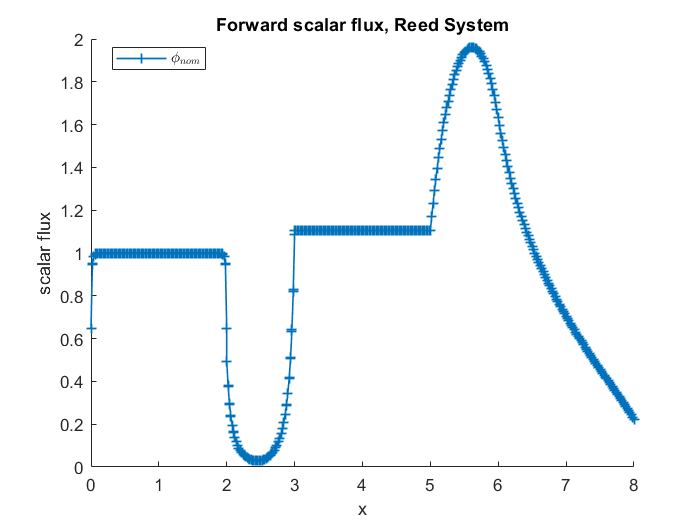
\includegraphics[width=0.6\linewidth]{phi_reed.png}
  \caption{Forward scalar flux solution of reed problem.}
\label{fig:phi_reed}
\end{figure}

As previously mentioned attempting to apply the VET adjoint-method to this system with the $0$ Eddington assumption produces unusable results. This is particularly bad when $\sigs$ is perturbed in regions $4$ and $5$.

\section{Proposal}
From my master's thesis work, a sensitivity formulation for the scalar flux using the first order adjoint applied to the VET formulation of the neutron transport equation is
\begin{equation}
\delta \qoi = \bra \delta \scalSource, \vefadj  \ket - \bra \delta \siga \phi, \vefadj \ket  - \bra \delta \isigt \div \left( \Edd^u \phi \right) , \grad \vefadj \ket + \sbra \vefadj, 2 \delta J^{\text{inc}} \sket - \bra  \isigt \div \left( \tcr{\delta \Edd} \phi \right), \grad \vefadj \ket
- \sbra \vefadj, \phi \tcr{\delta \BEdd} \sket .
\end{equation}
The problematic terms are highlighted in red, since we do not know the Eddington perturbation terms. Within my thesis I mainly assumed $\delta \Edd,\delta \BEdd=0$ which lead to problems for certain scenarios. I did a very quick and simple refinement to very simply compute a $\delta \Edd/ \delta p$ sensitivity for a parameter $p$ and add the term back in, which resulted in much stronger agreement between the VET sensitivity and transport sensitivity.

This leads me to think of the above formulation as a method which reduces the problem of transport UQ to a problem of an Eddington tensor UQ (which is of lower dimensionality). Working under the sort of general idea that the Eddington tensor is not very sensitive to may parameter perturbations, then hopefully applying a method such as POD where our interest is $\Edd$ results in a small relevant basis. Then with a ROM for predicting $\delta \Edd$ we can utilize that prediction in the $\delta \qoi$ formulation above and obtain a much better first order perturbation than was done in the thesis. Importantly due to solution dimensionality this method should be more memory feasible than performing POD on the full angular flux solution $\psi$. Moreover, since $\Edd$ doesn't depend on the response $q^\dag$, performing the POD for our system gets a $\delta \Edd$ prediction that can be used for ANY response function. For every new $\qoi$ we only need to perform one additional quasi-diffusion solve to gain $\vefadj$

So the general idea:
\begin{itemize}
\item Offline POD stage - use an SN solver to generate snapshots of $\Edd$. Computationally expensive. May end up being memory expensive but hopefully not as much as performing POD on $\psi$. May consider using a coarser mesh in this stage.
\item Online stage using the ROM to generate a $\delta \Edd$ value given system perturbations $\delta p$.
\item Using the found $\delta \Edd$ in the VET Adjoint inner-product for $\delta \qoi$ shown above.
\end{itemize}

The hope is that this results in a better prediction of $\delta \qoi$ than was found in my thesis, particularly for void problems. Also the limiting factor is to ensure that the memory doesn't requirement doesn't exceed that of performing an adjoint method using a full transport $\psi$.

\end{document}